% TeX root = main.tex

% First argument to \section is the title that will go in the table of contents. Second argument is the title that will be printed on the page.
\section[Lecture 3--{Surfaces in Space}]{3. Surfaces in Space}
There are two ways to study the curvature of a surface: (1)following Euler (1760), consider
the curvatures of all normal sections. (2) the derivative of unit normal vector fields.
In this section, we along the first way to define the curvature at a point on a surface.
Then we introdce Gauss's Theorema Egregium and Gauss-Bonnet theorem that are through out the whole
differential geometry.
Here, a surface in $\sR^3$ is treated as a \textbf{regular $2$-dimensional submanifold}.
We emphsize the regularity to gaurantee the surface is smooth and has no singular points.
\subsection{Principal, Mean, and Gaussian Curvatures}
A \textbf{normal vector} to $M$ at $p$ is a vector $N_p \in T_p \sR^3$
that orthogonal to the tangent plane $T_p M$. A normal vector field $N$ is a function that assigns
each $p$ a normal vector $N_p$
\begin{align}
    N_p = \sum_{i=1}^{3}a^i(p)\frac{\partial}{\partial x^i}\Bigg| _p .\nonumber
\end{align}
The $C^\infty$ of all $a^i(p)$ implies $N$ is a $C^\infty$ vector field.
\begin{figure}
    \centering
    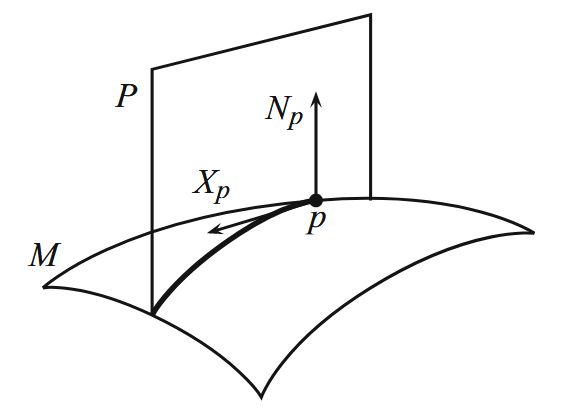
\includegraphics[width=0.5\textwidth]{../Lectures/Figures/norm_vector.png}
    \caption{Normal Section at $p$~\cite[p. 17]{tuDifferentialGeometry2017}.}
    \label{fig. norm vector}
\end{figure}
Let $N$ be a $C^\infty$ unit normal vector field, the plane $P$ that contains $N_p$ slice the
surface $M$ along a plane curve $P \cap M$ through $p$, as shown in Figure~\ref{fig. norm vector}.

By the \textbf{transversality theorem}~\cite{tu2010introduction}, 
$P \cap M$ is transversal, then being smooth. Such a plane curve is called \textbf{section} of
the surface through $p$. Suppose the normal sections has $C^\infty$ parameterizations, we can 
describe the how the surface curves at $p$ by the collection of all the curvatures at $p$ 
of all sections w.r.t. normal vector $N_p$.

Let $\gamma(s)$ be the normal section parameterized by arc length, which satisfies
$\gamma(0)=p$ and $\gamma'(0)=X_p$, where $X_p$ is a unit tangent vector, that determines the
normal vector $N_p$ and the orientation of $\gamma(s)$. Then, we can define the curvature of 
normal section $\gamma$ at $p$ w.r.t. $N_p$ by
\begin{align}
    \kappa(X_p)=\inner{\gamma''(0)}{N_p}. 
\end{align}
Since the set of all unit vectors $X_p$ is a unit circle,
we have a function $\kappa: S^1 \rightarrow \sR$. Since reverse the sign of $X_p$ does not change
the sign of second derivative of $\gamma$, $\kappa(-X_p)=\kappa(X_p)$.

The maximum and minimum value $\kappa_1, \kappa_2$ of $\kappa$ are the \textbf{principal curvatures} of the surface at $p$.
Their average $(\kappa_1 + \kappa_2) / 2$ is the \textbf{mean curvature} $H$.
Their product $\kappa_1 \cdot \kappa_2$ is the \textbf{Gaussian Curvature} $K$.
The unit tangent vector $X_p$ that corresponds to principal curvature is called
the \textbf{principal direction}.
\begin{remark}
    If we reverse the sign of unit normal vector to $-N_p$, the sign of curvature will change,
    but the Gaussian curvature stays, which means that the Gaussian curvature
    is \textbf{independent} of the choice of the unit normal vector field.
\end{remark}
\begin{example}[Sphere with a radius $a$]
    Recall the circle $S^1$ in Example~\ref{eg. circle}, every normal section is circle, then
    we have the principal curvature $1/a$,
    the mean curvature $H=1/2a$, the Gaussian curvature $K=1/{a^2}$.
\end{example}
\begin{example}
    For a cylinder of radius $a$ with a unit inward normal vector field (Figure~\ref{fig. cylinder}).
    The principal curvature $\kappa_1=1/a, \kappa_2=0$, the mean curvature $H=1/2a$,
    the Gaussian curvature $K=0$.
\end{example}
\begin{figure}
    \centering
    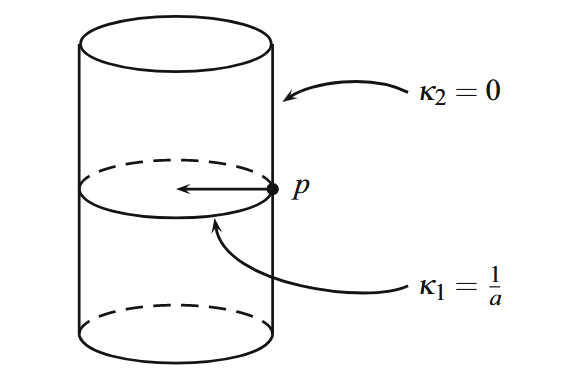
\includegraphics[width=0.5\textwidth]{../Lectures/Figures/cylinder.png}
    \caption{Principal curvatures of a cylinder~\cite[p. 19]{tuDifferentialGeometry2017}.}
    \label{fig. cylinder}
\end{figure}
\subsection{Gauss's Theorema Egregium}
$\kappa_1,\kappa_2$ is not invariant under the isometry, but the Gaussian curvature $K$ dose.
The Gauss's Theorema Egregium tells us that the Gaussian curvature is independent of the
embedding of the manifold, but the inherit geometry. This will be detailed in the following chapters.
\subsection{The Gauss--Bonnet Theorem}
The integral of Gaussian curvature gives a \textbf{topological invariant}, independent of
Riemannian metric. For example,
integral the Gaussian curvature $1/a^2$ of a sphere $S^2$ with radius $a$ gives $4\pi$.

For a compact oriented surface $M$ in $\sR^3$, the integral
\begin{align}
    \int_{M} K dS = 2\pi \chi(M), \nonumber
\end{align}
where $\chi(M)$ denotes the Euler characteristic.
\problemsection{Problems}
\begin{problem}
Suppose $M$ is a smooth surface in $\mathbb{R}^3$, 
$p$ a point in $M$, and $N$ a smooth unit normal vector field
 on a neighborhood of $p$ in $M$. Let $P$ be the plane spanned by a unit tangent vector 
 $X_p \in T_p M$ and the unit normal vector $N_p$. 
 Denote by $C := P \cap M$ the normal section of the surface $M$ at $p$ cut out by the plane $P$.

\begin{enumerate}
    \item[(a)] The plane $P$ is the zero set of some linear function $f(x,y,z)$. 
    Let $\tilde{f} \colon M \to \mathbb{R}$ be the restriction of $f$ to $M$. 
    Then the normal section $C$ is precisely the level set $\tilde{f}^{-1}(0)$. 
    Show that $p$ is a regular point of $\tilde{f}$, i.e., 
    that the differential $\tilde{f}_{*,p} \colon T_p M \to T_0 \mathbb{R}$ is surjective. 
    (Hint: Which map is $f_{*,p} \colon \mathbb{R}^3 = T_p \mathbb{R}^3 \to T_{f(p)} 
    \mathbb{R} = \mathbb{R}$? What is its kernel?)

    \item[(b)] Show that a normal section of $M$ at $p$ is a regular submanifold of dimension 
    one in a neighborhood of $p$. (Hint: Apply~\cite[Proposition 11.4]{tu2010introduction} 
    and the regular level set theorem~\cite[Theorem 9.9]{tu2010introduction}.)
\end{enumerate}
\end{problem}

\begin{problem}
    Show that if a curve $C$ in a smooth surface is a regular submanifold of dimension one 
    in a neighborhood of a point $p \in C$, 
    then $C$ has a $C^\infty$ parametrization near $p$. 
    (Hint: Relative to an adapted chart $(U, x^1, x^2)$ centered at $p$, 
    the curve $C$ is the $x^1$-axis. A $C^\infty$ parametrization of the $x^1$-axis 
    in the $(x^1, x^2)$-plane is $(x^1, x^2) = (t, 0)$.)
\end{problem}